\documentclass[12pt,a4paper]{article}
\usepackage[margin=2cm, left=1.5cm, right=1.5cm]{geometry}
\usepackage{amsmath, amssymb, amsthm}
\usepackage{fancyhdr}
\usepackage{mdframed}
\usepackage{enumerate}
\usepackage{graphicx}
\usepackage{float}

\pagestyle{fancy}
\fancyhf{}
\fancyhead[L]{113-1 Machine Learning}
\fancyhead[R]{Final Project}
\fancyfoot[C]{\thepage}
\setlength{\headheight}{15pt}

\usepackage{silence}
\WarningFilter{latexfont}{Font shape}
\WarningFilter{latexfont}{Some font shapes were not available}

\usepackage{xeCJK}
\setCJKmainfont[AutoFakeBold=true, AutoFakeSlant=true]{bkai00mp.ttf}
\setCJKmonofont[AutoFakeBold=true, AutoFakeSlant=true]{bkai00mp.ttf}
\setCJKsansfont[AutoFakeBold=true, AutoFakeSlant=true]{bkai00mp.ttf}

% remove all figures for faster compilation
% \usepackage[allfiguresdraft]{draftfigure}

\setlength\parindent{0pt}
\linespread{1.25}

\begin{document}
\begin{center}
  {\LARGE \bf HTML 2024 Final Project}\\[8pt]
  \textbf{Team:} How To Make Lasagna\\
  B12902119 胡祐誠
  B12902123 常洧丞
  B12902037 張聲元
  B11902139 洪佑全
\end{center}


\section{Introduction}


\section{Preprocessing}
\subsection{empty data filling}
From the dataset obtained, there are $5\%$ per column of data missing, which increases the hardness to predict and to feed the data into model.
To convert the data into all floating point numbers to the model is crucial for not having strings and nan to effect the training process. \\
For strings, we first find out that most of the strings represent the names of team and players.
For a machine learning model to recognize the teams and players which links advantages between teams and players are not feasible to achieve by dataset only with about $12000$ data yet $30$ teams and $900$ pitchers.
Thus, converting the strings of player names into averall winning probabilities has more statistical meanings. 
However, since there are only $30$ teams it is plausible to convert to either a one hot vector of size $30$ or floating point numbers indicating team winning probabilities.
For those empty values, we then have two approaches, first is to simply convert those empty values to $0$, and another is using auto encoder to prerpocess the data and to fill the holes in the data. \\

\subsubsection{zero mapping}
Since mapping all empty values to zero values is naive, yet it intuitively allows the model to perform properly in most of the prediction algorithms.
However, zero mapping has an issue that all of our models cannot pass the baseline, which the performance lingers about $54\%$ to $57\%$. \\
From the point of view that zero mapping allows the first-step data to be passed to the model, whereas, the mapping to zero may contain large bias to the original data.
All $5\%$ of data are marked to zero which considerabily affect the aggregation of data, namely too much bias.

\subsubsection{auto encoder}
To solve the problem arise from mapping all empty values to zero, we utilize the features of the auto encoder that it filters the essential features and discard the non-essential ones.
Since training of auto encoder is goal to rebuild the same data out of the extracted features, we can utilize it to generate data with no holes which are more likely to resemble the original data. \\
By auto encoder, we finally passed the baseline by simple DNN, which shows that mapping empty values to zero decreases the statistical meaning and model performance significantly.


\subsection{PCA data simplification}
A data too complex or having too many similar features distracts the model while training and often leads to overfitting or falling into local minima.
To solve the problem we use PCA on highly similar columns to reduces the complexity of training data by half. \\

Our method first finds all pair of Pearson corelation coefficients and perform disjoint set union on those pair of correlation coefficient absolute value higher than $0.5$.
Then, apply PCA on those set having element greater than 1, reduce their dimensions by half, then rebuild the data with PCA processed columns. \\

By doing such preprocess, we find out interesting pattern in the dataset.
Some of the data pairs are highly similar in a third rank polynomial pattern, shown as below figure \ref{fig:51-53} and figure \ref{fig:51-53r}.
Also, the below pairs of figure \ref{fig:29-129}, figure \ref{fig:29-129r} and figure \ref{fig:51-53}, figure \ref{fig:51-53r} are highly similar data with high $r^2$ values plotting together.
We can find out that zero mapping highly distracts the dataset by forming two protruding straight lines as in figure \ref{fig:29-129} and figure \ref{fig:51-53}.
Also, from the recovered data using auto encoder, we can eliminate the two perpendicular straight lines and results in a higher $r^2$ value in the same similar pair as in figure \ref{fig:29-129r} and figure \ref{fig:51-53r}.
However, auto encoder sometimes fails to fill the accurate data and leads to some data points very far away from the data cluster as in figure \ref{fig:51-53r} the left and right most points.


\begin{figure}[h]
    \centering
    \begin{minipage}{.4\textwidth}
        \centering
        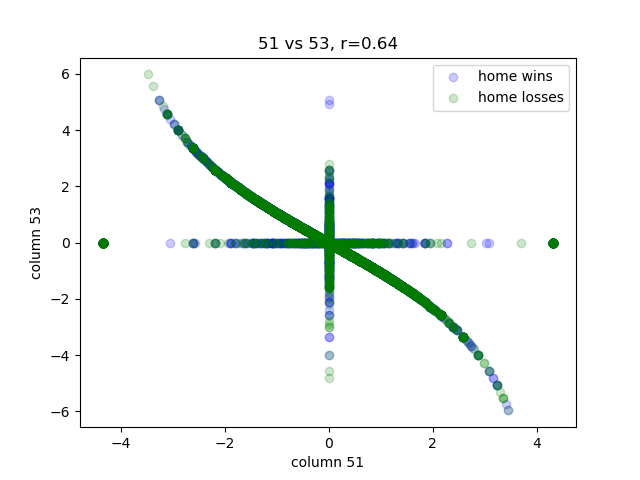
\includegraphics[width=0.8\linewidth]{0.64r_51_to_53.png}
        \caption[width=0.8\linewidth]{Column 51 to column 53 fill nan with zeros}
        \label{fig:51-53}
    \end{minipage}%
    \begin{minipage}{.1\textwidth}
        \ 
    \end{minipage}%
    \begin{minipage}{.4\textwidth}
        \centering
        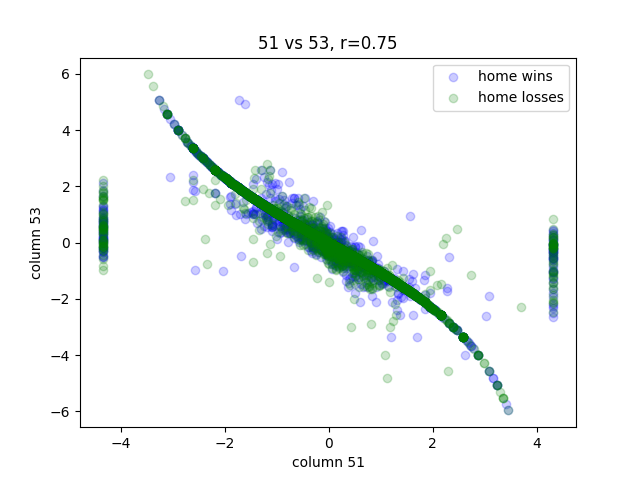
\includegraphics[width=0.8\linewidth]{0.75r_51_to_53_recovered.png}
        \caption[width=0.8\linewidth]{Column 51 to column 53 preprocess using auto encoder}
        \label{fig:51-53r}
    \end{minipage}

    \begin{minipage}{.4\textwidth}
        \centering
        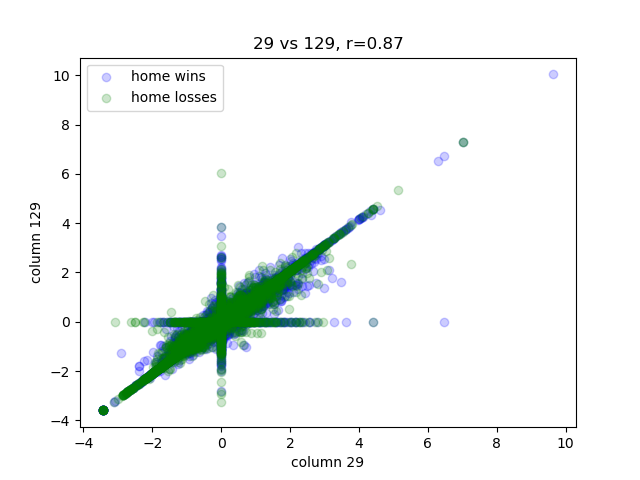
\includegraphics[width=0.8\linewidth]{0.87r_29_to_129.png}
        \caption[width=0.8\linewidth]{Column 29 to column 129 fill nan with zeros}
        \label{fig:29-129}
    \end{minipage}%
    \begin{minipage}{.1\textwidth}
        \ 
    \end{minipage}%
    \begin{minipage}{.4\textwidth}
        \centering
        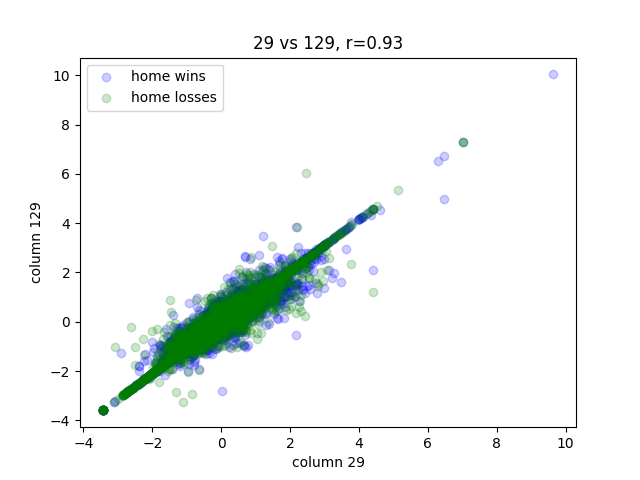
\includegraphics[width=0.8\linewidth]{0.93r_29_to_129_recovered.png}
        \caption[width=0.8\linewidth]{Column 29 to column 129 preprocess using auto encoder}
        \label{fig:29-129r}
    \end{minipage}
\end{figure}

After running the disjoint set union, we find out that there are $17$ goups of data to perform PCA, while two of the set has element over $10$ while others only has about $2$ to $4$ elements.
This may imply the dataset has numerous similar data columns that those columns represents the same or similar patterns and may cause training distraction, increase training time and performance cost.


\section{Model}

\subsection{Logistic Regression}

Logistic regression is the only approach we use that is in the MLF. We expect that it will be the least accurate one, but we still want to see how it performs. We used the preprocessed data to train the model, and split the data into 80\% training and 20\% validation. We trained the model 5000 times and choose the one with the highest validation accuracy for both stage 1 and stage 2. The highest validation accuracy we got in stage 1 was 0.64, and in stage 2 was 0.61. In spite of this, the performance of logistic regression in private was 0.56 in stage 1, and 0.53 in stage 2. Overall, logistic regression is one of the worst models we used in this project.

\subsection{Support Vector Machine}

\subsection{Random Forest}

\subsection{Neural Network}

\subsection{XGBoost}

\subsection{Clustering Methods}
In this project we tries to perform data splitting than assign the best arrangement of winning and losing on the data in the same cluster.
Since logistic regression, voting, DNN and most other method can be seen as seperating data points and the closest data will be assigned with the same win or lose.
Hence, we apply K-means clustering, Gaussian Mixture Model, and Mean Shift Clustering to cluster data points into different groups.
Then, we assign all groups with the $E_{in}$ maximizing output.
Hence, when prediction, the data point clustered into the specific groups will be assigned to the corresponding output identical to other data points in the same group.

\subsubsection{K-means Clustering}

\section{Result}

\section{Discussion}

\section{Reference}

\end{document}
